\documentclass{beamer}
\mode<presentation>
\usepackage{amsmath}
\usepackage{amssymb}
%\usepackage{advdate}
\usepackage{adjustbox}
\usepackage{subcaption}
\usepackage{enumitem}
\usepackage{multicol}
\usepackage{mathtools}
\usepackage{listings}
\usepackage{url}
\def\UrlBreaks{\do\/\do-}
\usetheme{Boadilla}
\usecolortheme{lily}
\setbeamertemplate{footline}
{
  \leavevmode%
  \hbox{%
  \begin{beamercolorbox}[wd=\paperwidth,ht=2.25ex,dp=1ex,right]{author in head/foot}%
    \insertframenumber{} / \inserttotalframenumber\hspace*{2ex} 
  \end{beamercolorbox}}%
  \vskip0pt%
}
\setbeamertemplate{navigation symbols}{}

\providecommand{\nCr}[2]{\,^{#1}C_{#2}} % nCr
\providecommand{\nPr}[2]{\,^{#1}P_{#2}} % nPr
\providecommand{\mbf}{\mathbf}
\providecommand{\pr}[1]{\ensuremath{\Pr\left(#1\right)}}
\providecommand{\qfunc}[1]{\ensuremath{Q\left(#1\right)}}
\providecommand{\sbrak}[1]{\ensuremath{{}\left[#1\right]}}
\providecommand{\lsbrak}[1]{\ensuremath{{}\left[#1\right.}}
\providecommand{\rsbrak}[1]{\ensuremath{{}\left.#1\right]}}
\providecommand{\brak}[1]{\ensuremath{\left(#1\right)}}
\providecommand{\lbrak}[1]{\ensuremath{\left(#1\right.}}
\providecommand{\rbrak}[1]{\ensuremath{\left.#1\right)}}
\providecommand{\cbrak}[1]{\ensuremath{\left\{#1\right\}}}
\providecommand{\lcbrak}[1]{\ensuremath{\left\{#1\right.}}
\providecommand{\rcbrak}[1]{\ensuremath{\left.#1\right\}}}
\theoremstyle{remark}
\newtheorem{rem}{Remark}
\newcommand{\sgn}{\mathop{\mathrm{sgn}}}
\providecommand{\abs}[1]{\left\vert#1\right\vert}
\providecommand{\res}[1]{\Res\displaylimits_{#1}} 
\providecommand{\norm}[1]{\lVert#1\rVert}
\providecommand{\mtx}[1]{\mathbf{#1}}
\providecommand{\mean}[1]{E\left[ #1 \right]}
\providecommand{\fourier}{\overset{\mathcal{F}}{ \rightleftharpoons}}
%\providecommand{\hilbert}{\overset{\mathcal{H}}{ \rightleftharpoons}}
\providecommand{\system}{\overset{\mathcal{H}}{ \longleftrightarrow}}
	%\newcommand{\solution}[2]{\textbf{Solution:}{#1}}
%\newcommand{\solution}{\noindent \textbf{Solution: }}
\providecommand{\dec}[2]{\ensuremath{\overset{#1}{\underset{#2}{\gtrless}}}}
\newcommand{\myvec}[1]{\ensuremath{\begin{pmatrix}#1\end{pmatrix}}}
\let\vec\mathbf

\lstset{
%language=C,
frame=single, 
breaklines=true,
columns=fullflexible
}

\numberwithin{equation}{section}

\title{1.10.20}
\author{Rushil Shanmukha Srinivas \\EE25BTECH11057 \\ Electrical Enggineering ,\\IIT Hyderabad.}

\date{\today} 
\begin{document} 

\begin{frame}
\titlepage
\end{frame}

\section*{Outline}
\begin{frame}
\tableofcontents
\end{frame}
\section{Problem}
\begin{frame}
\frametitle{Problem Statement}

Find the direction cosines of the line passing through the two points (-2,4,-5) and (1,2,3).
\\ \begin{table}[h!]    
  \centering
  \begin{center}
    \begin{tabular}{|c|c|c|} 
        \hline
            \textbf{Variable} & \textbf{Parameter} & \textbf{Value} \\ 
        \hline
            $\lVert \vec{B - A}\rVert$ & c & 5 cm \\ 
        \hline
             $\lVert \vec{C - B}\rVert$ & a & - \\ 
        \hline
             $\lVert \vec{C - A}\rVert$ & b &   -    \\
        \hline
            $\angle \vec{A}$  & -  & $45^\circ$ \\
        \hline
    \end{tabular}
\end{center}  

  \caption{Variables Used}
\end{table}
\end{frame}
\section{Solution}
\subsection{Echelon Form and Column Operations}
\begin{frame}
\frametitle{Echelon Form and Column Operations}
%\framesubtitle{Literature}
Let
\begin{align}
\vec{A}=\myvec {-2 \\ 4 \\ -5} ,\quad
\vec{B}=\myvec {1 \\ 2 \\ 3} .
\end{align}

Thus the direction (difference) vector of the line is
\begin{align}
\vec{v}=\vec{B}-\vec{A}=\myvec {3 \\ -2 \\ 8} .
\end{align}

\end{frame}

\subsection{Norm and Direction Cosines}
\begin{frame}
\frametitle{Norm and Direction Cosines}
 The length of $\vec{v}$ is
\begin{align*}
\vec{v}^\top \vec{v} &= \myvec{3 & -2 & 8}\myvec{3 \\ -2 \\ 8} \\
&= 3^3 + \brak{-2}^2 + \brak{8}^2 \\
&= 9 + 4 + 64 = 77
\end{align*}

Therefore, the norm of $\vec{v}$ is
\begin{align*}
\norm{\vec{v}} &\overset{\Delta}{=} \sqrt{\vec{v}^\top \vec{v}} = \sqrt{77} 
\end{align*} 

The unit vector in the direction of $\vec{v}$ is  

\begin{align*} 
\frac{\vec{v}}{\norm{\vec{v}}}
&= \frac{1}{\sqrt{77}}\myvec{3 \\ -2 \\ 8}
\end{align*}
\end{frame}
\begin{frame}
Let $\alpha,\beta,\gamma$ be the angles made by the line with the $x,y,z$ axes respectively.Then, the direction cosines are the elements of the above direction vector
\begin{align*}
\cos\alpha = \frac{3}{\sqrt{77}}, \quad
\cos\beta = -\frac{2}{\sqrt{77}}, \quad
\cos\gamma = \frac{8}{\sqrt{77}}
\end{align*}

\end{frame}
\subsection{Plots}
\begin{frame}
\frametitle{Plots}
\begin{figure}
\centering
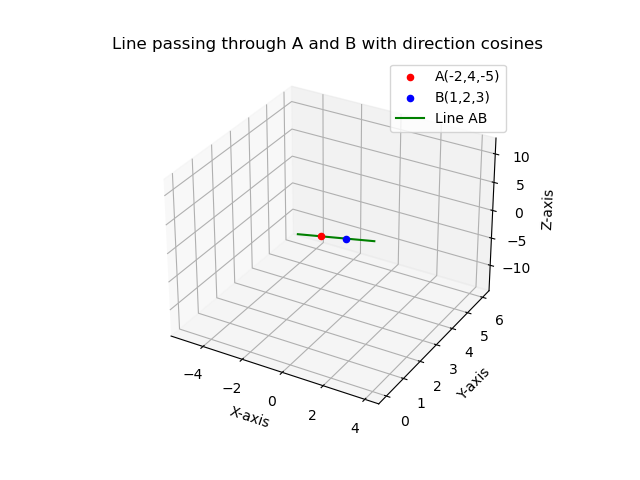
\includegraphics[width=0.7\columnwidth]{figs/fig_vector.png}
\caption{}
\label{fig:placeholder}
\end{figure}
\end{frame}
\section{C Code}
\begin{frame}[fragile]
\frametitle{C Code }
\begin{lstlisting}[language=C]
#include <stdio.h>
#include <math.h>

// Function to compute direction cosines between two 3D points
void direction_cosines(double x1, double y1, double z1,
double x2, double y2, double z2,
double *l, double *m, double *n) {
double dx = x2 - x1;
double dy = y2 - y1;
double dz = z2 - z1;
double mag = sqrt(dx*dx + dy*dy + dz*dz);

*l = dx / mag;
*m = dy / mag;
*n = dz / mag;
}
\end{lstlisting}
\end{frame}
\begin{frame}[fragile]
 \begin{lstlisting}[language=C]
        
// For testing in C directly
int main() {
double l, m, n;
direction_cosines(-2,4,-5, 1,2,3, &l,&m,&n);
printf("Direction cosines: (%lf, %lf, %lf)\n", l, m, n);
return 0;
}
\end{lstlisting}
\end{frame}

\section{Python Code}
\begin{frame}[fragile]
\frametitle{Python: call\_c.py}
\begin{lstlisting}[language=Python]
import ctypes

# Load the shared object
lib = ctypes.CDLL("./direction_cosines.so")

# Define argument and return types
lib.direction_cosines.argtypes = [
ctypes.c_double, ctypes.c_double, ctypes.c_double,
ctypes.c_double, ctypes.c_double, ctypes.c_double,
ctypes.POINTER(ctypes.c_double),
ctypes.POINTER(ctypes.c_double),
ctypes.POINTER(ctypes.c_double)
]

# Prepare variables
l = ctypes.c_double()
m = ctypes.c_double()
\end{lstlisting}
\end{frame}

\begin{frame}[fragile]
\begin{lstlisting}[language=Python]
n = ctypes.c_double()

# Call the function
lib.direction_cosines(-2, 4, -5, 1, 2, 3, ctypes.byref(l), ctypes.byref(m), ctypes.byref(n))

print("Direction cosines (C via .so):", (l.value, m.value, n.value))
    \end{lstlisting}
    \end{frame}
\begin{frame}[fragile]
\frametitle{Python Code for Plotting}
\begin{lstlisting}[language=Python]

import numpy as np
import matplotlib.pyplot as plt

# Given points
A = np.array([-2, 4, -5])
B = np.array([1, 2, 3])

# Direction ratios
AB = B - A
print("Direction ratios:", AB)

# Direction cosines
magnitude = np.linalg.norm(AB)
direction_cosines = AB / magnitude
print("Direction cosines:", direction_cosines)
\end{lstlisting}
\end{frame}
\begin{frame}[fragile]
    \begin{lstlisting}
# Plotting
fig = plt.figure()
ax = fig.add_subplot(111, projection='3d')

# Plot points A and B
ax.scatter(*A, color='red', label='A(-2,4,-5)')
ax.scatter(*B, color='blue', label='B(1,2,3)')

# Plot line passing through A and B
t = np.linspace(-1, 2, 100)  # parameter for line
line = A.reshape(3,1) + np.outer(AB, t)
ax.plot(line[0], line[1], line[2], color='green', label='Line AB')


# Labels
ax.set_xlabel('X-axis')
ax.set_ylabel('Y-axis')
ax.set_zlabel('Z-axis')
\end{lstlisting}
\end{frame}
\begin{frame}[fragile]
\begin{lstlisting}
ax.legend()
ax.set_title("Line passing through A and B with direction cosines")

plt.savefig("../figs/fig_vector.png")

plt.show()
\end{lstlisting}
\end{frame}

\end{document}
